\documentclass[12pt]{article}

% Packages
\usepackage{lastpage} 
\usepackage{fancyhdr}	%For header and footer
\usepackage{amsmath, amsthm, amssymb} %For mathematics
\usepackage{graphicx}
\usepackage{hyperref}	%For hyperlinks

% Page setup
\setlength{\topmargin}{-0.4in}
\setlength{\topskip}{0.3in}    % between header and text
\setlength{\textheight}{9.in} % height of main text
\setlength{\textwidth}{6.5in}    % width of text
\setlength{\oddsidemargin}{0in} % odd page left margin
\setlength{\evensidemargin}{0in} % even page left margin
\setlength{\parindent}{0pt}	% Suppress the indent

% Macros
\newcommand*{\bv}[1]{\textbf{#1}} % Write vectors in bold case within an equation environment

% Header and Footer
\pagestyle{fancy}%\fancyhead{}
\fancyhf{}	% Clear the default header and footer
\fancyhead[L]{MAE 3195 \\ Name:}
\fancyhead[R]{Credit Sheet 15 \\ \thepage /\pageref{LastPage}}


% Title
\title{MAE 3195, Credit Sheet 15\\ Introduction to Finite Element Method}
\date{}

% Body of document
\begin{document}
\maketitle

Write a Matlab code to solve the following problem. Use the discrete representation shown below:

\begin{figure}[htb]
	\begin{center}
		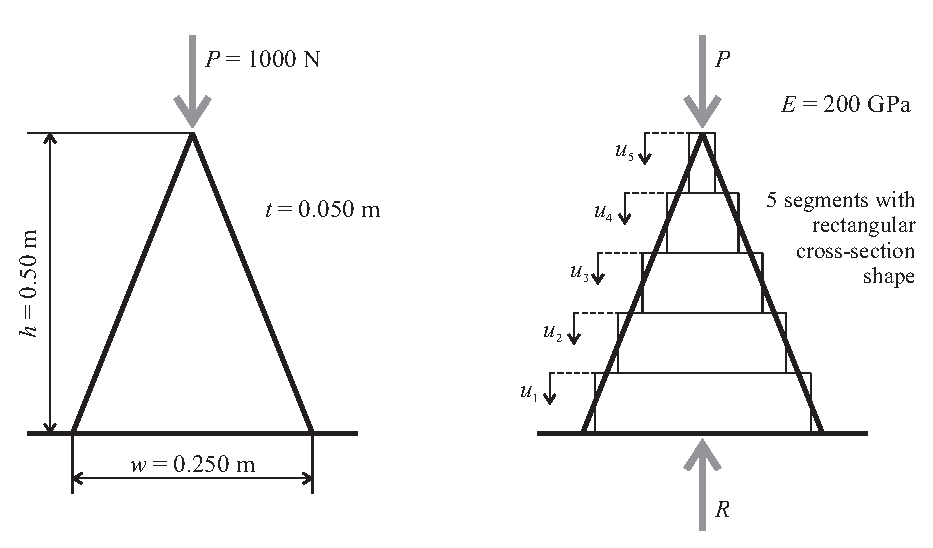
\includegraphics[width=6.in]{triangle.eps}
	\end{center}
\end{figure}

\begin{enumerate}
	\item Determine displacements $u_1$, $u_2$, ... $u_5$
	\item Determine reaction force, $R$
	\item Determine strain $\varepsilon_i$ in each segment
	\item Determine stress $\sigma_i$ in each segment.
\end{enumerate}

\end{document}